% Shared standalone design for the editable figure reconstructions.
\documentclass[tikz,border=5pt,10pt]{standalone}
\usepackage[T1]{fontenc}
\usepackage[utf8]{inputenc}
\usepackage{newpxtext,newpxmath}
\usepackage[scaled=.94]{sourcesanspro}
\usepackage{pgfplots}
\pgfplotsset{compat=1.18}
\usetikzlibrary{arrows.meta,calc,positioning,decorations.pathreplacing,
  decorations.markings,patterns,matrix,shapes.geometric,fit,backgrounds,
  intersections,angles,quotes}
\definecolor{ink}{HTML}{203746}
\definecolor{accent}{HTML}{146C78}
\definecolor{muted}{HTML}{667780}
\definecolor{signalred}{HTML}{B94B44}
\color{ink}
\tikzset{>=Latex,line width=.8pt,
  every node/.style={font=\small},
  axis/.style={->,draw=muted,line width=.5pt},
  guide/.style={draw=muted,dashed,line width=.45pt},
  curve/.style={draw=accent,line width=1pt},
  marker/.style={circle,fill=accent,inner sep=1.5pt},
  labelbox/.style={fill=white,inner sep=2pt}}

\begin{document}
\begin{tikzpicture}
\node[font=\small\sffamily]at(1,3.6){Projection onto a fixed set};
\path[fill=accent!9,draw=accent](0,0)--(2,0)arc[start angle=0,end angle=90,radius=2]--cycle;
\node at(.7,.8){$C$};
\foreach \p/\q in {{(-1,.9)}/{(0,.9)},{(1,-1.15)}/{(1,0)},{(-.9,-.9)}/{(0,0)},{(2.9,-.7)}/{(2,0)},{(-.7,2.9)}/{(0,2)}}{
\draw[->,muted]\p--\q;\fill[ink]\p circle(1.4pt);\fill[accent]\q circle(1.4pt);}
\draw[->,muted](2.3,2.3)--(1.4142,1.4142);\fill[ink](2.3,2.3)circle(1.4pt)node[above]{$x$};\fill[accent](1.4142,1.4142)circle(1.4pt)node[left]{$P_C(x)$};
\node[align=center,text width=5.3cm]at(.9,-2){$x-P_C(x)\in N_C(P_C(x))$};
\begin{scope}[shift={(7.2,.8)}]
\node[font=\small\sffamily]at(.2,2.8){A sublevel set determined by the input};
\node[font=\footnotesize]at(.2,2.3){$f(u,v)=\tfrac12(u^2+2v^2)$};
\pgfmathsetmacro{\levelradius}{sqrt(.7*.7+2*.45*.45)}
\pgfmathsetmacro{\levelminor}{\levelradius/sqrt(2)}
\path[fill=accent!7,draw=accent](0,0)ellipse({\levelradius} and {\levelminor});
\draw[accent!35](0,0)ellipse(.6 and .4243);
\draw[accent!35](0,0)ellipse(1.5 and 1.0607);
\draw[accent!35](0,0)ellipse(2 and 1.4142);
\coordinate(z)at(.7,.45);\coordinate(x)at(1.4,1.35);
\draw[->,signalred](x)--(z);\fill[ink](x)circle(1.5pt)node[above right]{$x$};\fill[accent](z)circle(1.5pt)node[below right]{$z$};
\node at(0,-.42){$C_x$};
\node[align=center,text width=6cm]at(.2,-2.8){$z=\operatorname{prox}_f(x)$,\quad $C_x=\{u:f(u)\leq f(z)\}$\\[6pt]$z=P_{C_x}(x)$};
\end{scope}
\end{tikzpicture}
\end{document}
